\chapter{Capturas de pantalla}
%En este capítulo puede mostrar capturas del sistema para que quede registro del avance del producto. Esta sección es opcional.
\section{Capturas de la funcionalidad Pantalla Principal}
%Recuerde poner un texto introductorio breve para cada sección.

En la figura se observa la vista de la aplicación al abrirla por primera vez, con disponibilidad del menú de "hamburguesa", el click derecho y la opción de abrir un PDF.

\vspace{1cm}
\begin{figure}[H]
  \centering
    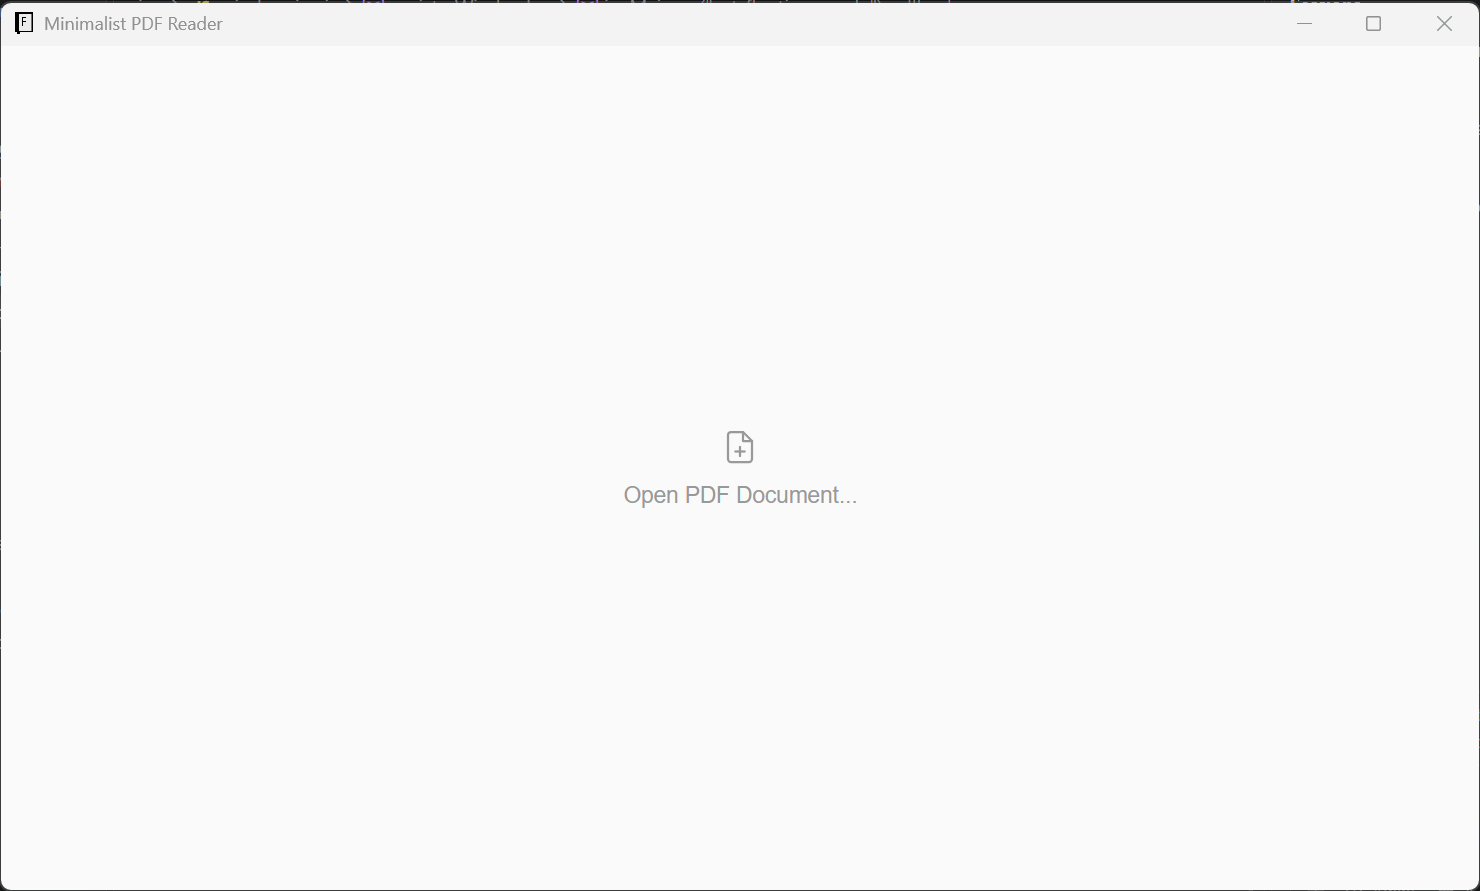
\includegraphics[height= 11cm, width=17cm]{project/images/Home.png}
\end{figure}

\section{Capturas de la funcionalidad Abrir PDF}
%No olvide referenciar las imágenes en el texto usando \emph{label} y \emph{ref}.

En la figura se observa la vista una vez abierto el archivo PDF, con los números de página y el menú de "hamburguesa".

\begin{figure}[H]
  \centering
    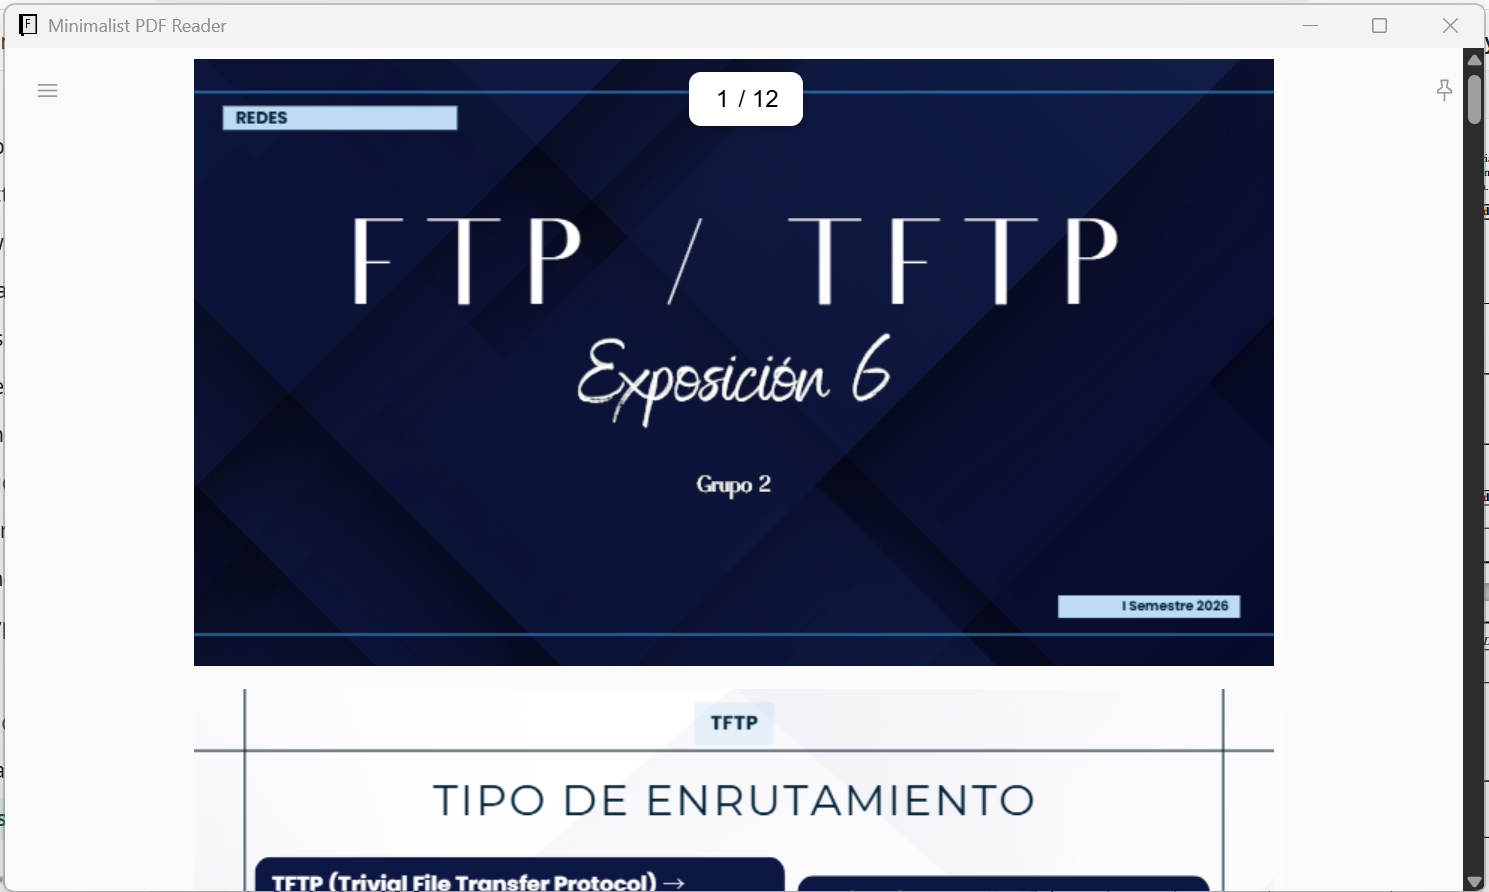
\includegraphics[height= 11cm, width=17cm]{project/images/openPDF.png}
\end{figure}